\documentclass{article}
\usepackage{arxiv}

\usepackage[utf8]{inputenc}
\usepackage[english, russian]{babel}
\usepackage[T1]{fontenc}
\usepackage{url}
\usepackage{booktabs}
\usepackage{amsfonts}
\usepackage{nicefrac}
\usepackage{microtype}
\usepackage{lipsum}
\usepackage{graphicx}
\usepackage{natbib}
\usepackage{doi}



\title{Биоидентификация планарий после декапитации}

\author{ Никифорова Мария Дмитриевна\\
	Факультет Вычислительной математики и кибернетики\\
	МГУ имени М. В. Ломоносова\\
	Москва, Россия \\
	\texttt{nikiforova.maria.d@gmail.com} \\
	%% examples of more authors
	\And
	  Местецкий Леонид Моисеевич \\
	Факультет Вычислительной математики и кибернетики\\
	МГУ имени М. В. Ломоносова\\
	Москва, Россия \\
	\texttt{mestlm@mail.ru} \\
	%% \AND
	%% Coauthor \\
	%% Affiliation \\
	%% Address \\
	%% \texttt{email} \\
	%% \And
	%% Coauthor \\
	%% Affiliation \\
	%% Address \\
	%% \texttt{email} \\
	%% \And
	%% Coauthor \\
	%% Affiliation \\
	%% Address \\
	%% \texttt{email} \\
}
\date{}

\renewcommand{\shorttitle}{Биоидентификация планарий после декапитации}

%%% Add PDF metadata to help others organize their library
%%% Once the PDF is generated, you can check the metadata with
%%% $ pdfinfo template.pdf
\hypersetup{
pdftitle={Биоидентификация планарий после декапитации},
pdfsubject={q-bio.NC, q-bio.QM},
pdfauthor={Никифорова Мария Дмитриевна},
pdfkeywords={Распознавание изображений},
}

\begin{document}
\maketitle

\begin{abstract}
	В настоящей работе предлагается метод для персональной
идентификации особей отряда планарии. 
Планарии известны своей способностью к регенерации и являются популярной биологической моделью. 
Идентификация отдельных особей планарий полезна для автоматизации биологических исследований и повышения точности измерений в экспериментах. 
В работе предлагается метод идентификации планарий по их текстурному профилю, который характеризует набор, форму и расположение светлых пятен на теле червя — участков без пигмента.
Предложеннный метод ставит целью решить задачу идентификации планарии после декапитации(отсечения головной части). 
\end{abstract}


\keywords{Распознавание изображений \and Задача о назначениях \and Computer vision}

\section{Introduction}

Пресноводные плоские черви planaria являются классической биологической моделью. Способность взрослых планарий к морфогенезу, то есть к регенерации и бесполому
размножению, является наиболее выраженной в
животном мире \cite{int1} \cite{int2}. 
Планарии - единственные животные в мире, которые способны восстанавливать свою центральную нервную систему и головной нервный узел, и этот процесс происходит за очень короткое время, от одной до трех недель. 
Развитие цифровых технологий для создания и
анализа изображений позволило разработать
количественное описание морфогенеза планарии in vivo \cite{int3} \cite{int4}.
Планарии также являются одним из потенциально многообещающих
объектов в изучении клеточных основ иммунитета,
который у планарий протекает путем фагоцитоза пищи
всеми клетками планарии, за исключением нервных и половых клеток. 
Учитывая нынешний интерес к различным биологическим моделям
, связанным с проблемами клеточного иммунитета, планарии могут стать одной из перспективных моделей для изучения фагоцитоза in vivo \cite{int5} \cite{int6} \cite{int7}.
Однако широкому использованию планарий для
решения различных фундаментальных и прикладных
задач препятствует ряд нерешенных объективных проблем,
одной из которых является проблема идентификации
особей планарий в ходе эксперимента.
Особенностью биологии бесполой расы планарий
Girardia tigrina является их предпочтение к групповому обитанию
во время экспериментов. 
Кроме того,
планарии этого вида, сидящие в одиночестве, как правило, размножаются через 24 часа, что мешает проведению достаточно длительных
экспериментов, поэтому во время эксперимента таких
планарий содержат в группе из 25-30 особей, чтобы
ограничить бесполое размножение \cite{int8} \cite{int5}.
Однако при групповом содержании
невозможно отличить планарий друг от друга, что ограничивает возможность оценки состояния индивидуальных характеристик протекания
определенных физиологических процессов в течение нескольких дней.
В этой работе была предпринята попытка идентифицировать планарий на
основе особенностей структуры поверхности их тела. 
Видовое название планарий, Girardia
tigrina, связано с пятнистой структурой их поверхности. Это обстоятельство дает возможность использовать особенности текстуры поверхности тела
отдельных планарий в качестве основы для их
персональной идентификации.
Это позволит оценить динамику морфогенеза и
фагоцитоза планарий in vivo, что даст основу для создания количественных моделей течения этих биологических процессов.
Такие модели, в свою очередь,
будут полезны при изучении возможностей управления
длительными сложными биологическими процессами на уровне
всего организма.

\section{Постановка задачи}
Имеется набор изображений особей отряда планарии до декапитации(отсечения головы) и после.
Требуется научиться идентифицировать особей в процессе регенерации.

\end{section}

\section{Данные}
Датасет для решения задачи состоит из 579 изображений планарий. В датасете представлены изображения 20 особей. Для каждой особи есть 5 или 6 её изображений до декапитации и от 4 до 8 изображений через 1, 2, 3, 4, 6 или 10 дней после декапитации. Изображения нормализованы: планарии сегментированы, их форма и размер стандартизованы. Размер изображений составляет $1024 \times 144$ пикселя, расширение - .png, цветовая модель - RGB. \ref{fig:fig1}

\begin{figure}[H!]
\centering
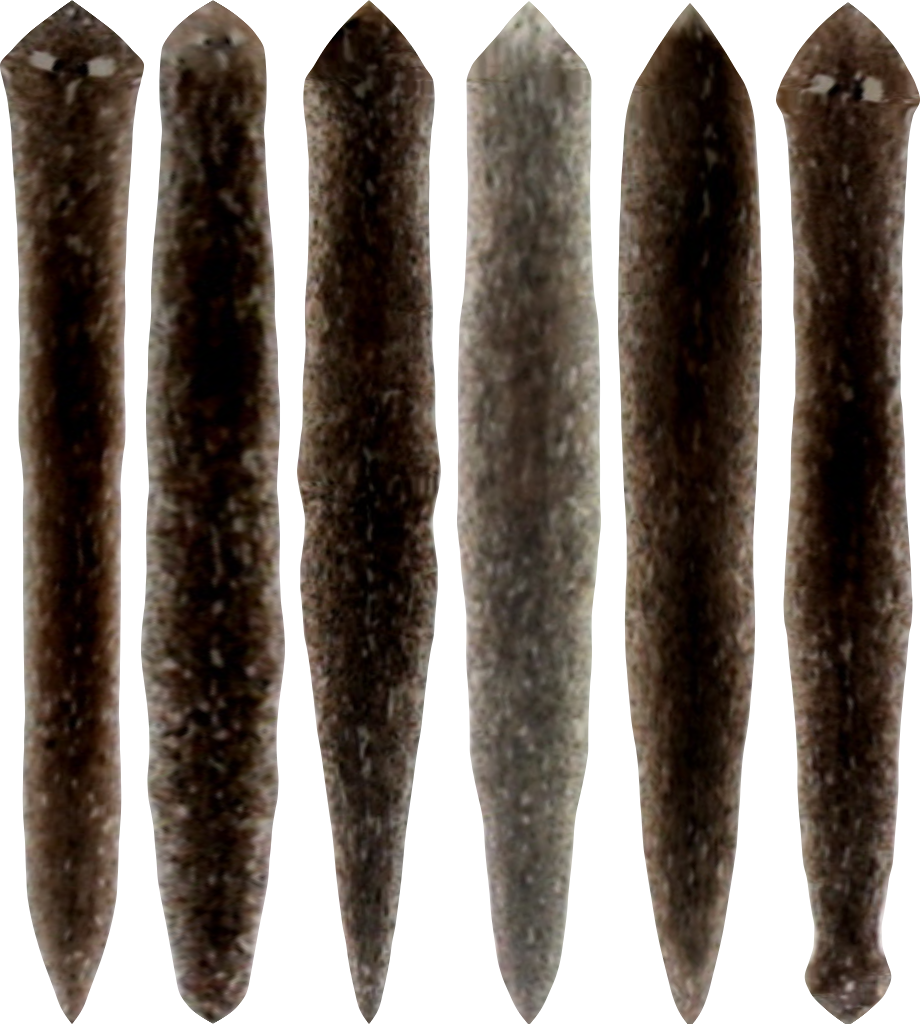
\includegraphics[scale=0.4]{examples.png}
\centering
\caption{Примеры входных данных}
\label{fig:fig1}
\end{figure}


\begin{section}{Метод решения}

Идея решения основывается на следующем наблюдении: пятна эпителия светлого цвета на поверхности тела планарии имеют довольно стабильную топологическую структуру, по которой можно попробовать отличить особей. \ref{fig2}

\begin{figure}[H]
\centering
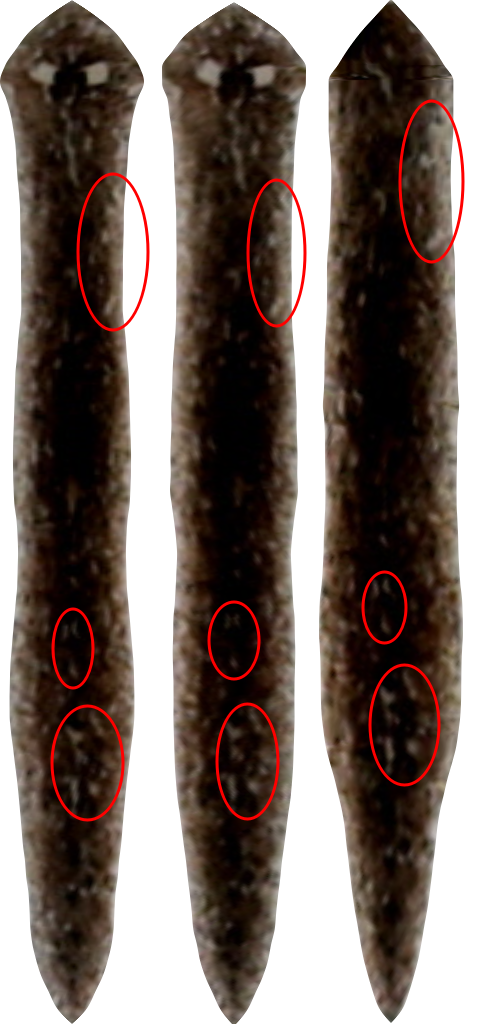
\includegraphics[scale=0.4]{character.png}
\caption{Пример стабильных фрагментов текстуры планарии}
\label{fig2}
\end{figure}

Предлагается выделить светлые пятна с изображения, отобрать среди них наиболее стабильные и характерные, составить из них шаблон путём усреднения, и проводить идентификацию на основе сравнения новых текстурных профилей с шаблоном.

\begin{subsection}{Извлечение текстурного профиля}

    Для того, чтобы выделить участки светлого пигмента, изображение переводилось в оттенки серого. Далее к нему применялся фильтр Гаусса с параметром $\sigma = 2$, затем вычислялся Лапласиан и снова применялся фильтр Гаусса с параметром $\sigma=1$. После этого проводилась бинаризация по порогу 200. Чтобы удалить артефакты, связанные с краевыми эффектами, но не несущие значимой информации, выделялись связанные компоненты и отбрасывались те из них, которые имели пересечение с фоном.
    Также из результирующего текстурного профиля отбрасывались пятна, которые имели площадь менее 5 пикселей.
    \ref{fig3}

\begin{figure}[H]
\centering
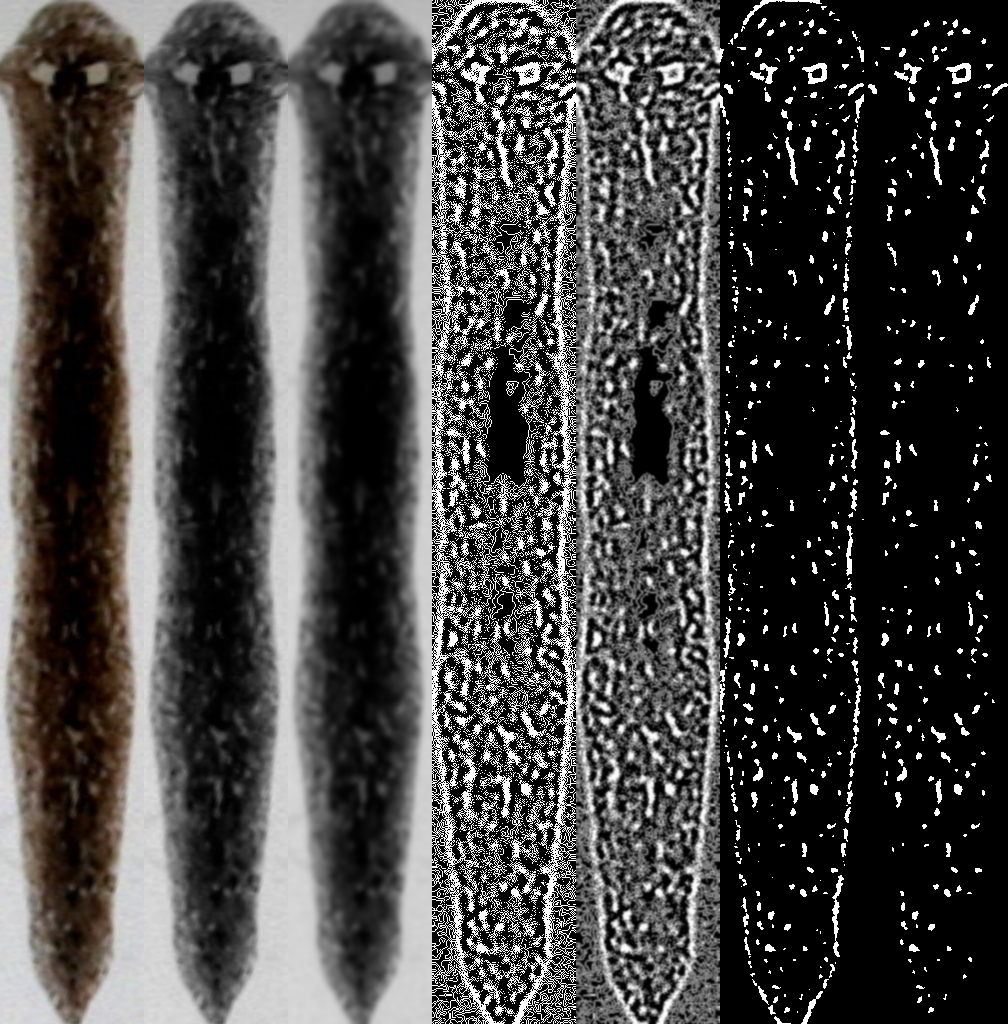
\includegraphics[scale=0.3]{spots_extraction.png}
\centering
\caption{Пример выделения текстурного профиля планарии. (1) - исходное изображение, (2) - изображение в оттенках серого, (3) - после применения фильтра Гаусса, (4) - после вычисления Лапласиана, (5) - после применения второго фильтра Гаусса, (6) - бинаризация, (7) - удаление лишних артефактов}
\label{fig3}
\end{figure}
    
\end{subsection}

\begin{subsection}{Сравнение паттернов пятен}

Теперь будем рассматривать задачу сопоставления пятен двух текстурных профилей одной особи.

Наивное наложение изображений друг на друга в данном случае будет давать плохой результат, так как даже в рамках одного дня группы пятен флуктуируют.
Поэтому зададим меру сходства двух пятен и будем искать на её основе оптимальное с точки зрения суммарного сходства сопоставление. \ref{fig4}

\begin{figure}[H]
\centering
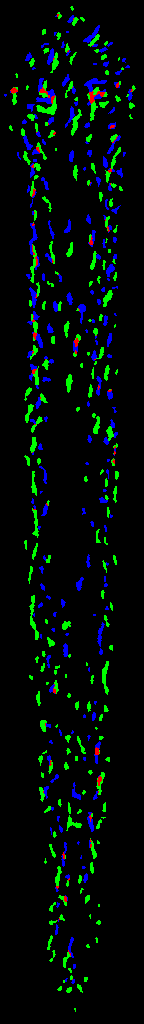
\includegraphics[scale=0.3]{intersection.png}
\caption{Пример, когда два текстурных профиля одной и той же планарии в рамках одного дня практически не имеют пересечений(синий и зеленый цвета соответствуют двум разным изображениям, красным отмечено их пересечение)}
\label{fig4}
\end{figure}

Запишем формально задачу сопоставления паттернов пятен для двух планарий. Пусть у первой особи количество выделенных пятен равно $n$, у второй - $m$. Тогда мы хотим сопоставить пятну на первой планарии пятно на второй планарии, принимая во внимание следующие факты:

\begin{itemize}
    \item Большое значение имеет координата центра пятна
    \item Цельное пятно на одной планарии может соответствовать нескольким разным близкорасположенным пятнам на другой планарии, но таких пятен не может быть больше двух
    \begin{figure}[H]
    \centering
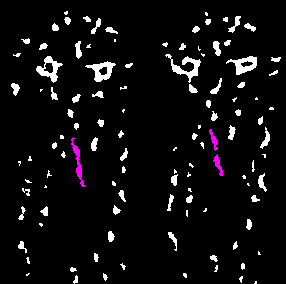
\includegraphics[scale=0.7]{split.png}
\caption{Пример, когда цельное пятно соответствует двум раздельным пятнам}
\end{figure}
    \item Часто существенную роль играет не только расположение пятна, но еще и его форма
    \item Некоторые пятна могут остаться несопоставленными, но всего должно быть найдено хотя бы $k$ пар
\end{itemize}

Таким образом, получаем следующую оптимизационную задачу:\\
\begin{gather*}
\sum_{i, j}{c_{ij}a_{ij}} \rightarrow min \\
\sum_{i=1}^{n}a_{ij} \leq 2 \\
\sum_{j=1}^{m}a_{ij} \leq 2 \\
\sum_{i, j}a_{ij} \geq k \\
a_{ij} \in \{0, 1\}, c_{ij} \in \RR
\end{gather*}

где $c_{ij}$ - мера того, насколько сильно i-е пятно первого профиля отличается от j-го пятна второго профиля. В данной задаче \[c_{ij} = dist(center_i, center_j) +  10 * (1 - IoU(spot_i, spot_j))\]
, где $dist(center_i, center_j)$ - евклидово расстояние между центрами масс пятен, $IoU(spot_i, spot_j)$ - Intersection over Union для двух пятен. 

    
\end{subsection}

\begin{subsection}{Идентификация планарий}

Идентификация планарий основывается на сравнении с эталоном каждой особи и выбором в качестве ответа той, суммарное совпадение с которой максимально.
В данной работе в качестве эталона берется так называемый \textit{паспорт} планарии.

\begin{subsubsection}{Построение паспорта}

Будем называть \textit{паспортом} планарии изображение того же размера, что и остальные фотографии, полученное путём обобщения текстурных профилей и выделения наиболее характерных паттернов для конкретной планарии.

Паспорт строится путём последовательного сопосталения текстурных профилей планарии до декапитации и включения в паспорт пятен, расположенных на середине отрезка, соединяющего два найденных пятна, и имеющих форму объединения двух сопоставленных пятен.

\end{subsubsection}

\begin{subsubsection}{Линейное преобразование}

Для того, чтобы сопоставить изображение планарии после декапитации с изображением нулевого дня, необходимо задать преобразование для местоположения пятен, так как после декапитации паттерны пятен смещаются относительно тела планарии. \ref{fig5}
\begin{figure}[H]
\centering
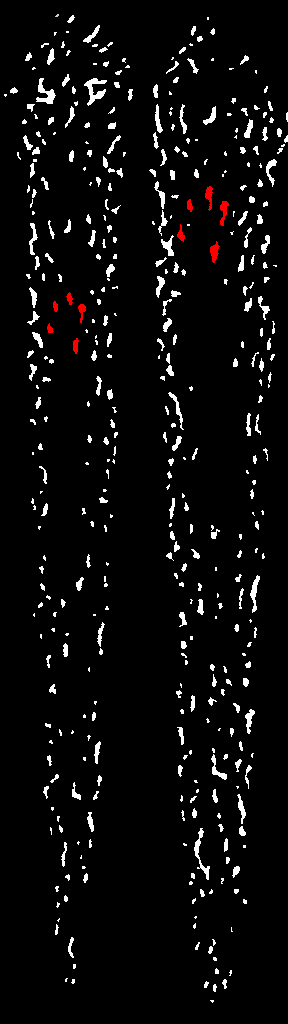
\includegraphics[scale=0.3]{linear.png}
\caption{Пример смещения паттернов пятен на изображении при декапитации планарии}
\label{fig5}
\end{figure}

Для решения этой проблемы предлагается сжимать изображение вдоль вертикальной оси относительно самой нижней хвостовой точки на коэффициент $\alpha$, конкретное значение которого подбирается путём перебора для обеспечения наилучшего сопоставления с паспортом. В данном случае использовался перебор параметра $\alpha$ по сетке $[0.9, 0.91, ..., 0.99, 1.0]$. Так как коэффициент сжатия небольшой, то форма пятен также меняется незначительно. Такие изменения сопоставимы с неточностями при извлечении текстурного профиля.
После сжатия изображение сверху дополняется нулями. Эта область соответствует области отсечённой головы.
    
\end{subsubsection}

Таким образом, полная процедура идентификации планарии выглядит следующим образом:

\begin{enumerate}
    \item Построение паспортов всех планарий по изображениям до декапитации
    \item Поиск подходящего коэффициента $\alpha
    $
    \item Сравнение сжатого текстурного профиля планарии со всеми паспортами, выбор среди них того, с которым сходство максимально.
\end{enumerate}
    
\end{subsection}

\end{section}

\begin{section}{Эксперименты}

Рассмотрим распределение меры сходства на примере двух хороших с точки зрения качества изображений планариях.

В качестве меры сходства берётся суммарная площадь пересечения всех пятен с паспортом. \ref{ref6}

\begin{figure}[H]
\centering
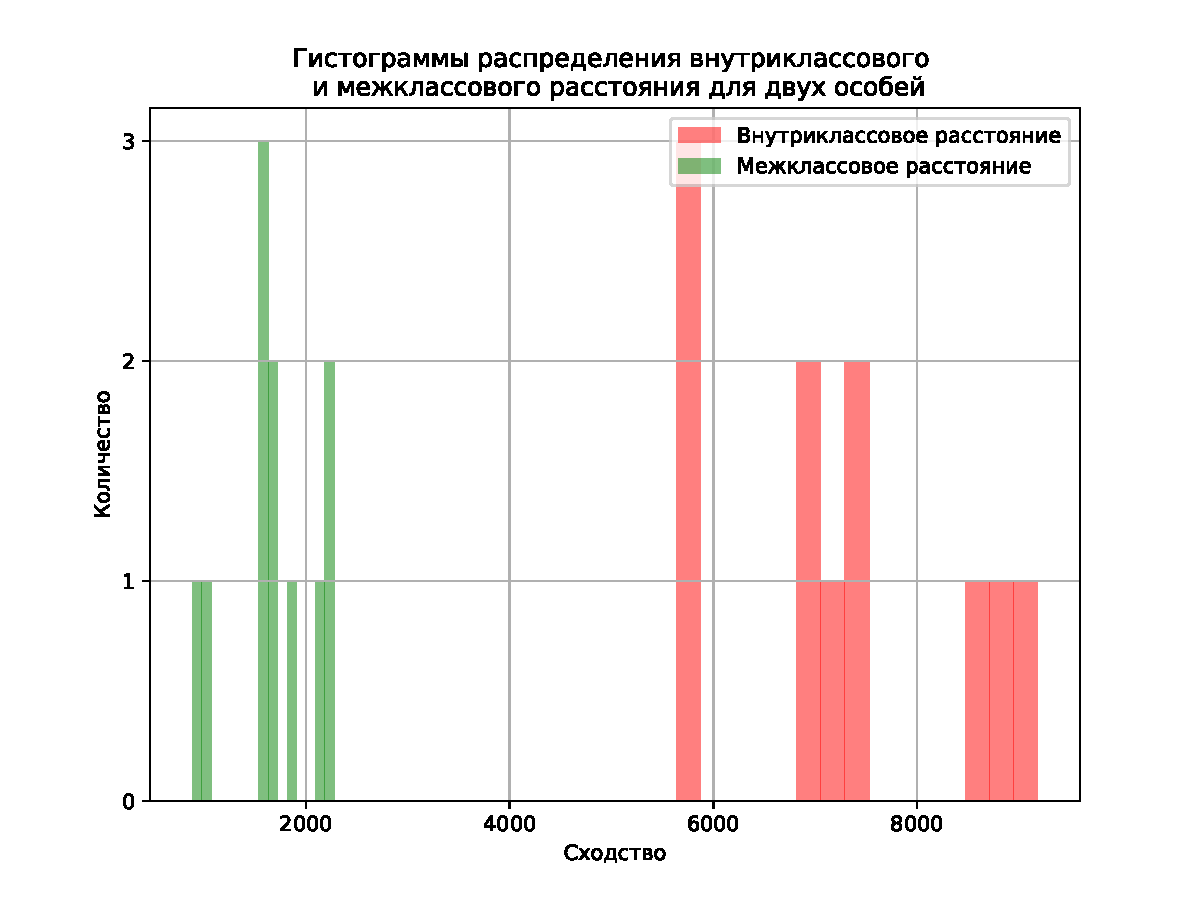
\includegraphics[scale=0.7]{hist-1.pdf}
\label{ref6}
\end{figure}

Как видно по графику, в данном случае можно выставить порог для принятия решения об отношении планарии к данному классу равным, например, 4000, и в таком случае идентификация будет верной.

Теперь посмотрим на распределение сходства для двух планарий, у которых качество исходных изображений другое. \ref{fig7}

\begin{figure}[H!]
\centering
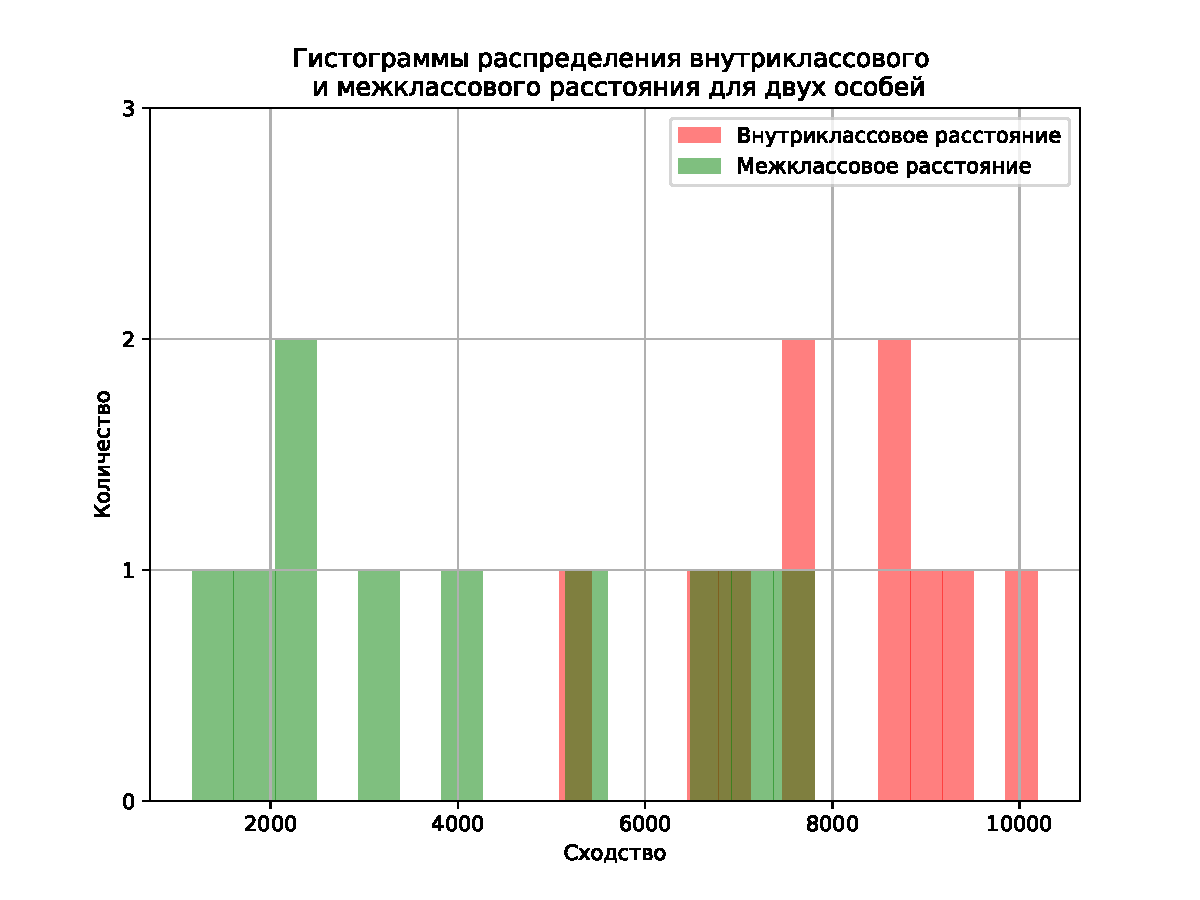
\includegraphics[scale=0.7]{hist_bad.pdf}
\label{fig7}
\end{figure}

Подобные распределения, когда невозможно выставить порог, четко разделяющий классы, возникают либо когда текстурный профиль содержит слишком много пятен, либо когда исходное изображение некачественное, и пятен наоборот выделяется слишком мало. \ref{fig8}

\begin{figure}[H!]
\centering
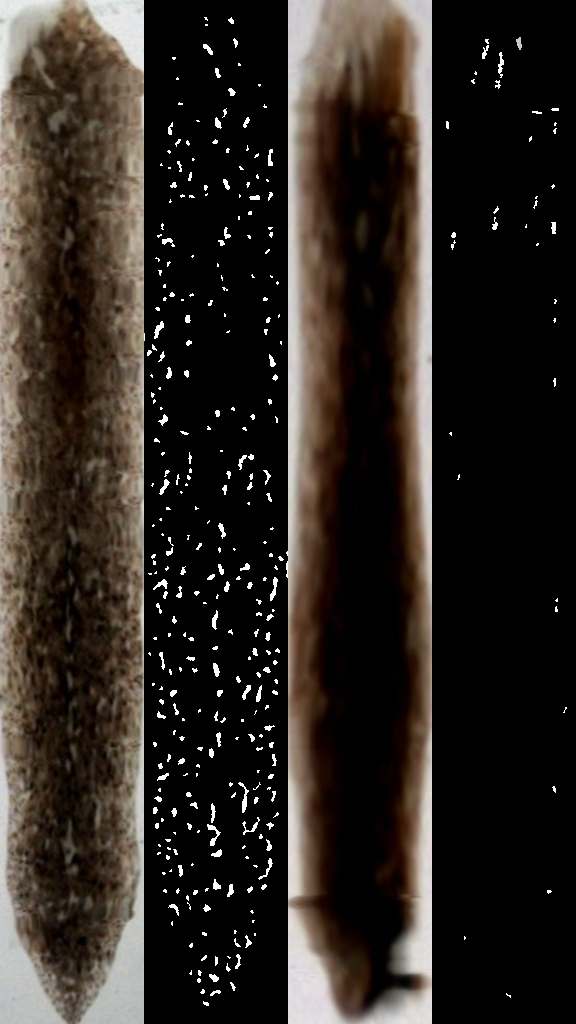
\includegraphics[scale=0.3]{lessmore.png}
\caption{Пример фотографии и выделенного текстурного профиля одной и той же планарии во 2 и 6 дни после декапитации}
\label{fig8}
\end{figure}

\end{section}

\bibliographystyle{unsrtnat}
\bibliography{references}

\end{document}
